\documentclass{report}

\usepackage{graphicx}
\graphicspath{ {./images/} }
\usepackage[utf8]{inputenc}
\usepackage[T1]{fontenc}
\usepackage{float}
\usepackage{geometry}
 \geometry{
   a4paper,
   left=30mm,
   top=30mm,
}
\usepackage{pdflscape}
\usepackage[cyr]{aeguill}
\usepackage{xspace}
\usepackage[french]{babel}
\usepackage{lmodern}
\usepackage{amsmath}
\usepackage[htt]{hyphenat}
\usepackage{xcolor}
\usepackage{listings}
\lstset{
  basicstyle=\ttfamily,
  columns=fullflexible,
  frame=single,
  breaklines=true,
  postbreak=\mbox{\textcolor{red}{$\hookrightarrow$}\space},
}

\begin{document}

Voici la function python représentant l'equation différentiel du mouvement de la voiture:\\
\begin{lstlisting}[language=Python]
def eq_diff_voiture(t,x,d,Db,Df,b,l,meq):
    p=0.055
    Cr=3.3e-4
    k=0.092
    theta_0=4.615
    req=1/(2/Db+2/Df)
    
    theta = x[0]
    theta_d = x[1]

    x_d = theta_d
    x_dd = 1/np.sin(theta)*(-theta_d**2*np.cos(theta)+np.sqrt(b**2+l**2-2*b*l*np.cos(theta))*(theta_d**2*b*l*np.sin(theta)**2/((b**2+l**2-2*b*l*np.cos(theta))**(3/2))+d/(meq*Db*b*l)*(-k*(theta-theta_0)*d*np.sqrt(b**2+l**2-2*b*l*np.cos(theta))/(Db*b*l*np.sin(theta))-Cr/req-p*Db*b*l/d*theta_d*np.sin(theta)/(np.sqrt(b**2+l**2-2*b*l*np.cos(theta))))))

    return np.array([x_d, x_dd])
\end{lstlisting}
Afin de résoudre cette équation différentielle, nous avons utilisé la méthode de Runge-Kutta d'ordre 4, grâce à la fonction \texttt{solve\_ivp} de la librairie \texttt{scipy.int} :\\
\begin{lstlisting}[language=Python]
def solve_eq_diff_voiture(params):
    t_i ,t_f = 0, 15
    return solve_ivp(eq_diff_voiture, [t_i, t_f], [0.1, 0], args=(params['d'], params['Db'], params['Df'], params['b'], params['l'], params['meq']), t_eval=np.linspace(t_i, t_f, 50))    
\end{lstlisting}
Nous avons ensuite écris deux fonctions, l'une \texttt{calculate\_speed\_from\_sol} permettant de calculer la vitesse de la voiture à partir de la solution de l'équation différentielle, et l'autre \texttt{calculate\_time\_to\_reach\_length} permettant de calculer le temps nécessaire pour que la voiture atteigne une certaine distance (dans notre cas 15m). Voici le graphe de la vitesse de la voiture en fonction du temps avec les paramètres de la voiture faite au premier semestre :\\
\begin{figure}[h]
    \centering
    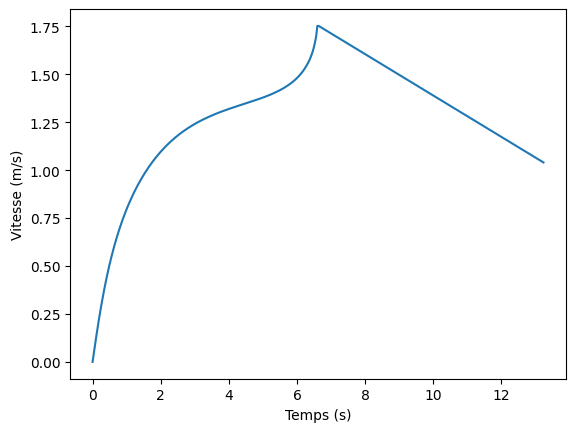
\includegraphics[width=0.8\textwidth]{vitesse_temps}
    \caption{Vitesse de la voiture en fonction du temps}
\end{figure}
On obtient par ailleurs un temps de 11.6s pour que la voiture atteigne les 15m. Désormais il faut optimiser les paramètres de la voiture pour qu'elle atteigne les 15m en moins de temps possible. Nous avons donc tenté de minimiser le temps de parcours en utilisant la fonction \texttt{minimize} de la librairie \texttt{scipy.optimize} cependant la fonction comportait trop de minimum locaux ou de plateau pour que l'optimisation soit efficace. C'est pour cette raison que nous nous sommes tourné vers la fonction \texttt{differential\_evolution} de la même librairie. Cette fonction permet de trouver le minimum global d'une fonction en utilisant un algorithme évolutionnaire. Le principe est de générer une population de points aléatoires dans l'espace des paramètres, puis de les faire évoluer en les faisant se reproduire et muter. Voici la fonction que nous avons utilisé pour optimiser les paramètres de la voiture : \\
\begin{lstlisting}[language=Python]
    bounds = [
        (3e-3, 0.1),  # d
        (0.03, 0.3),  # Db
        (0.03, 0.3),  # Df
        (0.03, 0.5),  # b
        (0.03, 0.5),  # l
    ]
    
    def objective(X):
        params = {
            'd': X[0],
            'Db': X[1],
            'Df': X[2],
            'b': X[3],
            'l': X[4]
        }
        sol = solve_eq_diff_voiture(params)
        v, t = calculate_speed_from_sol(sol, params)
        return calculate_time_to_reach_length(v, t, 15)
    
    def find_optimal_params():
        def callback(x, convergence):
            mc, meq = masse_vehicule(x[1], x[2], x[4])
            print(f'x: {x}, convergence: {convergence}, meq: {meq}, mc: {mc}')
    
        x0 = [0.00559557,0.14238863,0.15014371,0.12704067,0.12638812]
        return differential_evolution(objective, bounds=bounds, x0=x0,callback=callback, disp=True, workers=-1, updating='deferred',maxiter=100)
    
    opt = find_optimal_params()
    print(opt)
    
    optimal_params = {
        'd': opt.x[0],
        'Db': opt.x[1],
        'Df': opt.x[2],
        'b': opt.x[3],
        'l': opt.x[4],
    }
    
    sol = solve_eq_diff_voiture(optimal_params)
    v, t = calculate_speed_from_sol(sol, optimal_params)
    plot_speed(v, t)
    print(calculate_time_to_reach_length(v, t, 15))
\end{lstlisting}
On a d'ailleurs spécifié des bornes pour les paramètres afin de guider l'algorithme vers des valeurs raisonnables. On a également utilisé la fonction \texttt{callback} pour afficher les valeurs des paramètres à chaque itération de l'algorithme. On obtient finalement un temps de 9.8s pour que la voiture atteigne les 15m. Voici le graphe de la vitesse de la voiture en fonction du temps avec les paramètres optimaux: \\
\begin{figure}[h]
    \centering
    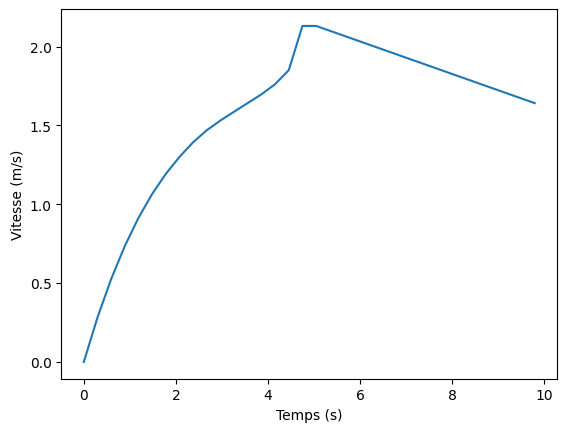
\includegraphics[width=0.8\textwidth]{vitesse_temps_optimal}
    \caption{Vitesse de la voiture en fonction du temps avec les paramètres optimaux}
\end{figure}
Nous avons du faire quelques optimisations afin d'obtenir un temps de convergences raisonnables (quelques dizaines de minutes). Par exemple nous avons utilisé l'argument \texttt{workers=-1} pour utiliser tous les processeurs et ainsi accélérer l'algorithme, d'autre part dans la résolution de l'equation différentielle nous avons utilisé un pas de temps de 50 points pour accélérer la convergence étant donné que la fonction \texttt{solve\_ivp} est la fonction la plus coûteuse en temps de calcul à chaque itération.

\end{document}